\documentclass[11pt,a4paper]{article}

% -----------------------------------------------------
% Packages
% -----------------------------------------------------
\usepackage[utf8]{inputenc}
\usepackage[T1]{fontenc}
\usepackage{xcolor}
\usepackage{geometry}
\usepackage{multicol}
\usepackage{amsmath, amssymb}
\usepackage{tikz}
\usetikzlibrary{positioning}
\usepackage{tcolorbox}
\usepackage{enumitem}
\usepackage{hyperref}
\usepackage{titlesec}
\usepackage{lmodern}
\usepackage{array}
\usepackage{colortbl}
\usepackage{graphicx}

% -----------------------------------------------------
% Styling
% -----------------------------------------------------
\geometry{top=1.5cm, bottom=1.5cm, left=1.5cm, right=1.5cm}
\setlength{\columnsep}{0.8cm}

\definecolor{myblue}{RGB}{48, 84, 150}
\definecolor{mygreen}{RGB}{0, 140, 90}
\definecolor{myred}{RGB}{180, 40, 40}
\definecolor{lightgray}{RGB}{245,245,245}
\definecolor{darkgray}{RGB}{220,220,220}
\definecolor{orange}{RGB}{255, 136, 0}

\titleformat{\section}
  {\normalfont\Large\bfseries\color{myblue}}{}{0em}{}

\titleformat{\subsection}
  {\normalfont\bfseries\color{mygreen}}{}{0em}{}

\hypersetup{
    colorlinks=true,
    linkcolor=myblue,
    urlcolor=myred,
}

\tcbset{
    colback=lightgray,
    colframe=myblue,
    boxrule=0.8pt,
    arc=3pt,
    left=5pt,
    right=5pt,
    top=5pt,
    bottom=5pt
}

% -----------------------------------------------------
% Document
% -----------------------------------------------------
\begin{document}

% ---------------- Title ----------------
\begin{center}
    {\huge \bfseries \color{myblue} Bregman Divergence}\\[0.2cm]
    {\large \color{mygreen} A Geometric and Philosophical Summary}
\end{center}

\vspace{0.4cm}
\begin{multicols}{2}

% ---------------- Section 1 ----------------
\section{1. Core Definition}

Let \( F : \mathbb{R}^n \to \mathbb{R} \) be a strictly convex, differentiable function.

The \textbf{Bregman divergence} between \( p \) and \( q \) is defined as:
\[
D_F(p \parallel q) = F(p) - F(q) - \langle \nabla F(q),\, p - q \rangle
\]

\begin{tcolorbox}
It measures how much \( F(p) \) lies above the linear approximation of \( F \) at \( q \).
\end{tcolorbox}

\textbf{Key properties:}
\begin{itemize}[leftmargin=0.6cm]
  \item Non-negative: \( D_F(p \parallel q) \ge 0 \)
  \item Zero iff: \( p = q \)
  \item Generally asymmetric
  \item Not a metric, but geometrically meaningful
\end{itemize}

% ---------------- Section 2 ----------------
\section{2. Geometric Insight}

\begin{center}
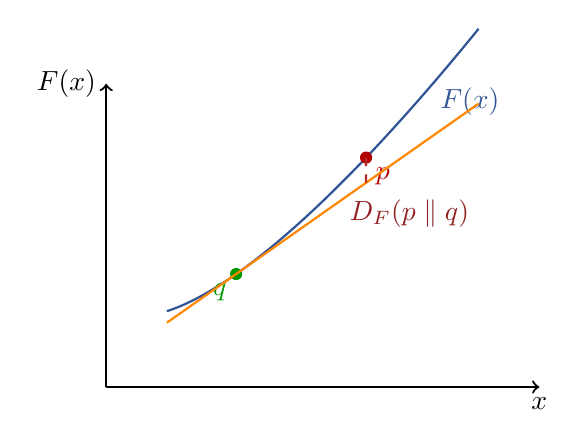
\begin{tikzpicture}[scale=1.1]
    \draw[->, thick] (0,0) -- (5,0) node[below] {\(x\)};
    \draw[->, thick] (0,0) -- (0,3.5) node[left] {\(F(x)\)};

    \draw[myblue, thick, domain=0.7:4.3, samples=100] plot (\x,{0.5*\x*ln(\x)+1});
    \node[myblue] at (4.2,3.3) {\(F(x)\)};

    \coordinate (q) at (1.5,{0.5*1.5*ln(1.5)+1});
    \coordinate (p) at (3,{0.5*3*ln(3)+1});

    \fill[green!60!black] (q) circle (2pt) node[below left] {\(q\)};
    \fill[red!70!black] (p) circle (2pt) node[below right] {\(p\)};

    % Tangent line
    \draw[orange, thick, domain=0.7:4.3] 
      plot (\x, { (0.5*1.5*ln(1.5)+1) + (0.5*ln(1.5)+0.5)*(\x-1.5) });

    % Vertical dotted line
    \draw[myred, dashed, thick] (3,{0.5*1.5*ln(1.5)+1+(0.5*ln(1.5)+0.5)*(3-1.5)}) -- (p);

    \node[myred!80!black] at (3.5,2.0) {\(D_F(p\parallel q)\)};
\end{tikzpicture}
\end{center}

\vspace{0.3cm}
\noindent
This gap represents the divergence. The greater the curvature, the more costly a linear approximation becomes.

% ---------------- Section 3 ----------------
\section{3. Convexity Condition}

\textbf{Jensen's inequality:}
\[
F(\lambda x + (1-\lambda)y) \le \lambda F(x) + (1-\lambda) F(y)
\]

\textbf{Differential form:}
\[
\nabla^2 F(x) \succeq 0
\]

This ensures that the function lies above all its tangents — a requirement for divergence to be non-negative.

% ---------------- Section 4 ----------------
\section{4. Interpretations}

\begin{itemize}[leftmargin=0.5cm]
  \item \( p \): true object, data point, or target
  \item \( q \): model, approximation, or belief
  \item Divergence is the extra cost of using \( q \) to model \( p \)
\end{itemize}

\begin{tcolorbox}
Divergence = \emph{Tension between truth and its approximation}
\end{tcolorbox}

% ---------------- Section 5 ----------------
\section{5. Optimization Role}

Bregman divergence guides algorithms like:

\begin{itemize}[leftmargin=0.5cm]
  \item Mirror descent
  \item Online learning and regret minimization
  \item Variational methods
\end{itemize}

\[
\min_q \int D_F(p(x)\parallel q(x))\,dx
\]

\end{multicols}

% ---------------- Section 6 ----------------
\section{6. Bayesian Connection}

When \( F(p) = \int p(x)\log p(x)\,dx \), we recover:

\[
D_F(p\parallel q) = D_{KL}(p\parallel q)
\]

\begin{itemize}
  \item KL divergence is a Bregman divergence
  \item Natural geometry of exponential families
  \item Variational Bayes: minimizes KL to approximate posterior
\end{itemize}

\begin{tcolorbox}
Bregman divergence underlies belief revision in Bayesian inference.
\end{tcolorbox}

% ---------------- Section 7 ----------------
\section{7. Summary Table and Diagram}

\vspace{0.2cm}

\begin{center}
\renewcommand{\arraystretch}{1.6}
\setlength{\tabcolsep}{10pt}
\rowcolors{2}{gray!10}{white}
\begin{tabular}{|p{3.8cm}|p{4.8cm}|p{4.8cm}|}
\hline
\rowcolor{myblue!30}
\textbf{Perspective} & \textbf{Role of \(F\)} & \textbf{Meaning of \(D_F(p \parallel q)\)} \\
\hline
Convex analysis & Curvature generator & Gap from tangent to function \\
\hline
Inference theory & Loss function & Extra cost of modeling truth \\
\hline
Optimization & Descent geometry & Regret, update penalty \\
\hline
Information theory & Entropy engine & KL divergence \\
\hline
Bayesian inference & Posterior structure & Divergence in belief updates \\
\hline
\end{tabular}
\end{center}

\vspace{1cm}

% ---------------- TikZ Mind Map ----------------
\begin{center}
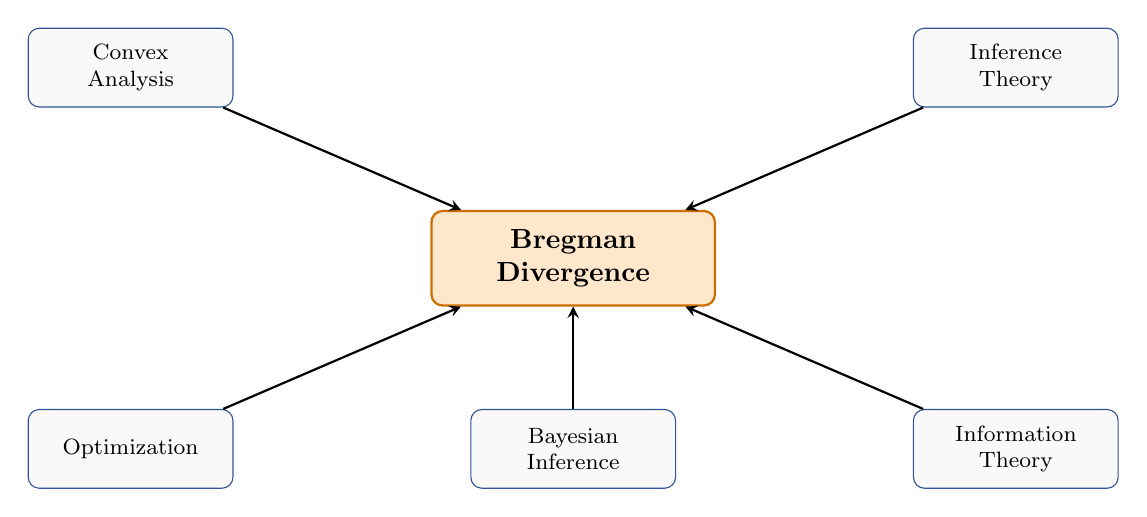
\begin{tikzpicture}[
    node distance=1.3cm and 2.5cm,
    concept/.style={rectangle, draw=myblue, fill=lightgray!60, rounded corners, font=\footnotesize, align=center, minimum width=2.6cm, minimum height=1cm},
    center/.style={rectangle, draw=orange!80!black, fill=orange!20, thick, rounded corners, font=\normalsize\bfseries, align=center, minimum width=3.6cm, minimum height=1.2cm},
    arrow/.style={->, thick, >=stealth}
]

\node[center] (core) {Bregman\\Divergence};

\node[concept, above left=of core] (convex) {Convex\\Analysis};
\node[concept, above right=of core] (inference) {Inference\\Theory};
\node[concept, below left=of core] (opt) {Optimization};
\node[concept, below right=of core] (info) {Information\\Theory};
\node[concept, below=of core] (bayes) {Bayesian\\Inference};

\draw[arrow] (convex) -- (core);
\draw[arrow] (inference) -- (core);
\draw[arrow] (opt) -- (core);
\draw[arrow] (info) -- (core);
\draw[arrow] (bayes) -- (core);

\end{tikzpicture}
\end{center}

\vspace{1cm}

\begin{center}
\textit{Bregman divergence is the geometric glue across learning, inference, and optimization.}
\end{center}

% ---------------- END ----------------
\end{document}